\section{Results}


\subsection{Historical Operation of \gls{EU} Reactors}


\begin{table}[h]
	\centering
	\scalebox{0.86}{
		\begin{tabular}{|c|c|c|}
			\hline
			Category  & Value [t] & Specifics \\ \hline
			Total Natural U & 1,314,003 & \\ \hline
			Total UOX Usage  & 188,196  &  \\ \hline
			Total MOX Usage  & 118 & \\ \hline
			Total Spent UOX  & 183,992 & \\ \hline
			Total Spent MOX  & 0 & All is Reprocessed. \\ \hline
			Total Tailings  & 1,125,798 & \\ \hline
		\end{tabular}}
		\caption{Simulation Results}
		\label{tab:sim_result}
		\end {table}

\Cref{tab:sim_result} lists the important metrics
obtained from the first simulation. The following
values are the \gls{EU} inventory and history at year 2050.


\begin{figure}[htbp!]
	\begin{center}
		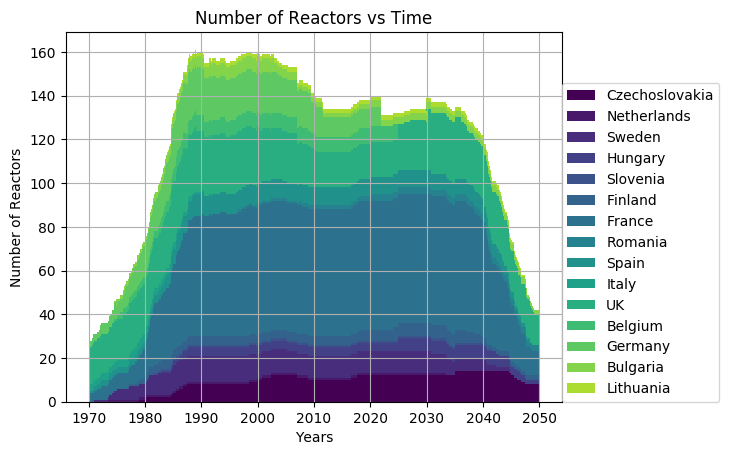
\includegraphics[width=\columnwidth]{./images/eu_future/number_plot.png}
	\end{center}
	\caption{Timeseries of number of reactors in \gls{EU}.}
	\label{fig:eu_num}
\end{figure}

\begin{figure}[htbp!]
	\begin{center}
		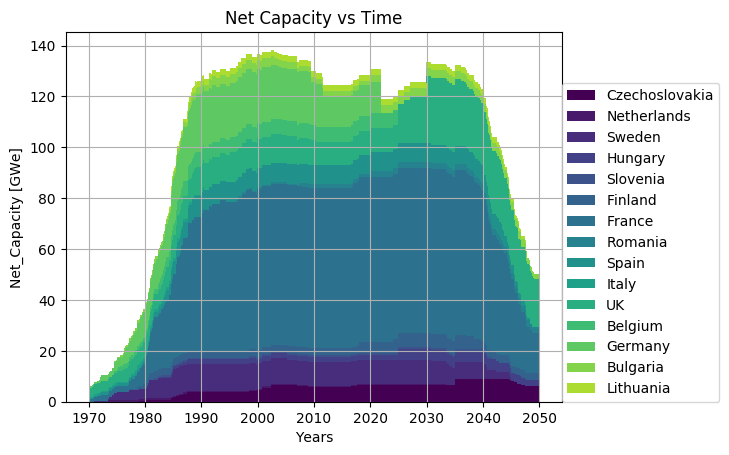
\includegraphics[width=\columnwidth]{./images/eu_future/power_plot.png}
	\end{center}
	\caption{Timeseries of installed nuclear capacity in \gls{EU}.}
	\label{fig:eu_pow}
\end{figure}

Figures \ref{fig:eu_num} and \ref{fig:eu_pow} display the
timeseries of number of reactors and installed capacity in \gls{EU}.

Figures \ref{fig:eu_tail} and \ref{fig:eu_snf} show the 
timeseries of mass of tailings and spent fuel accumulation in \gls{EU}.

\begin{figure}[htbp!]
	\begin{center}
		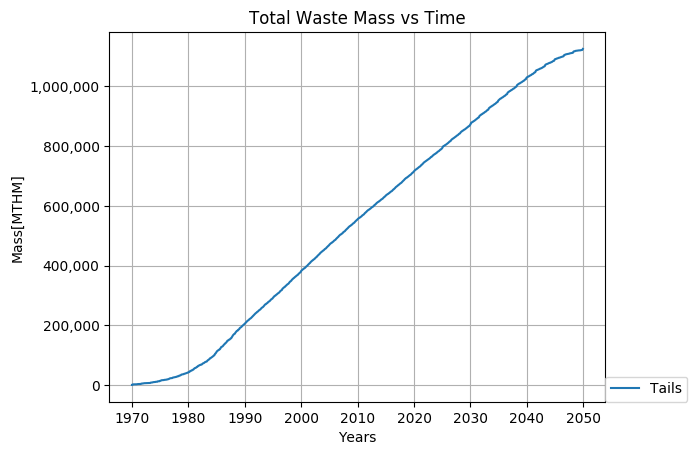
\includegraphics[width=\columnwidth]{./images/eu_future/tailings.png}
	\end{center}
	\caption{Timeseries of Tailings in the \gls{EU}.}
	\label{fig:eu_tail}
\end{figure}


\begin{figure}[htbp!]
	\begin{center}
			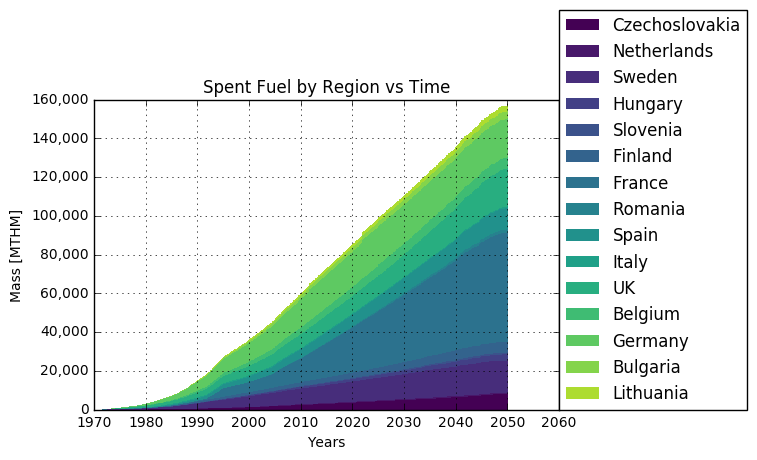
\includegraphics[width=\columnwidth]{./images/eu_future/snf.png}
	\end{center}
	\caption{Timeseries of Spent Nuclear Fuel in Sink.}
	\label{fig:eu_snf}
\end{figure}

\begin{table}[h]
	\centering
	\begin{tabular}{|c|c|c|}
		\hline
		Isotope & Mass Fraction in Spent Fuel [\%] & Quantity [t] \\ \hline
		Total & .9358 & 1,721.79 \\ \hline
		Pu238 & .0111 & 20.42 \\ \hline
		Pu239 & .518 & 953.07 \\ \hline
		Pu240 & .232 & 426.86 \\ \hline
		Pu241 & .126 & 231.82 \\ \hline
		Pu242 & .0487 & 89.6 \\ \hline
	\end{tabular}
	\caption{Plutonium From Spent Fuel}
	\label{tab:pu}
\end{table}


To create \gls{MOX}, ~9\% Pu and ~91\% depleted uranium is used.
Thus $1,721$ tons of plutonium yields $19,122$ tons of
\gls{MOX}. \Cref{tab:pu} lists the isotope, mass fraction,
and quantity of plutonium that can be obtained from the 2050 \gls{SNF} inventory.


\subsection{French \gls{SFR} Transition Scenario}

From Varaine et al., a French
ASTRID-type \gls{SFR} of capacity $600 MWe$ needs $1.225$ tons of
plutonium a year, with an initial plutonium loading of $4.9$ tons
\cite{marsaultmarie-sophie_pre-conceptual_2012}.
Thus, it can be assumed that the ASTRID reactor takes in $49$ tons of 
\gls{MOX}, and refuels a quarter of its fuel every year. Simply,
an ASTRID reactor needs $12.25$ tons of \gls{MOX} per year. 

The number of SFR-years worth of fuel that can be created with
the \gls{SNF} from 2050 is $\frac{19,122t}{12.25} = 1,560 $,
assuming infinite reprocessing and \gls{MOX} fabrication capacity.

However, assuming that \gls{MOX} can be recycled indefinitely,
spent \gls{MOX} from an ASTRID reactor
contains enough plutonium to produce a \gls{MOX} fuel with
the same mass, if mixed with depleted uranium. 
Separating plutonium from spent \gls{MOX} from
an ASTRID reactor can create \gls{MOX} 
the mass of spent \gls{MOX}, given sufficient tailings supply.

The second scenario, with the tails and spent \gls{UOX}
inventory, evaluates if the French can transition into \gls{SFR}
without constructing additional \gls{LWR}s. This simulation
assumed infinite reprocessing and fabrication capacity.

\Cref{fig:fuel} shows the mass of \gls{MOX} used in the 
\gls{SFR}s separated by how they are made, over time.
Note that the mass of \gls{MOX} from the spent \gls{UOX}
stops increasing around 2050, which means that the spent
\gls{MOX} is enough to create the \gls{MOX} for the
\gls{SFR} fleet. 

\begin{figure}[htbp!]
	\begin{center}
		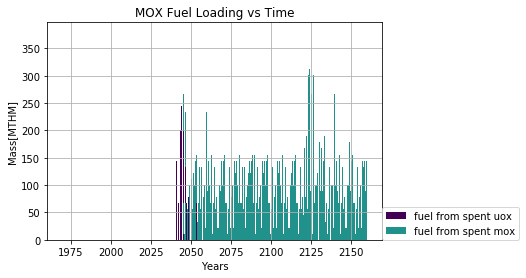
\includegraphics[width=\columnwidth]{./images/french-transition/where_fuel.png}
	\end{center}
	\caption{Timeseries of fuel used in the \gls{SFR}s [tons]}
	\label{fig:fuel}
\end{figure}

\Cref{fig:pu_demand} shows the separated plutonium demand
for \gls{MOX} production to fuel the ASTRID reactors given the deployment schedule.



\begin{figure}[htbp!]
	\begin{center}
		\includegraphics[width=\columnwidth]{./images/french-transition/pu_total_demand.png}
	\end{center}
	\caption{Separated Plutonium demand for \gls{MOX} production}
	\label{fig:pu_demand}
\end{figure}


\begin{table}[h]
	\centering
	\scalebox{0.86}{
		\begin{tabular}{|c|c|c|}
			\hline
			Category [unit] & Value & Specifics \\ \hline
			Total MOX used [t] & 164,141 & \\ \hline
			Total MOX from UOX Waste [t] & 19,136.2  &   \\ \hline
			Total MOX from MOX Waste [t] & 145,004.8 & \\ \hline
			Total Tailings used [t] & 149,368.3 & \\ \hline
			Total legacy SNF reprocessed [t] & 183,992 & \\ \hline
		\end{tabular}}
		\caption {\gls{SFR} Simulation Results}
		\label{tab:sfr_sim_result}
\end {table}


